\documentclass[tikz,border=6pt]{standalone}
\usepackage[T1]{fontenc}\usepackage{newtxtext,newtxmath}\usepackage{tikz}
\usetikzlibrary{arrows.meta,positioning,calc}
\definecolor{ink}{HTML}{172033}\definecolor{greyLine}{HTML}{9CA3AF}
\definecolor{greyFill}{HTML}{F3F4F6}\definecolor{qkC}{HTML}{B91C1C}
\definecolor{ovC}{HTML}{0B7285}
\tikzset{>={Latex[length=1.7mm 1.0,width=1.5mm 1.0]},
  posarr/.style={-{Latex[length=1.9mm 0.8,width=1.7mm 0.8]},line cap=round},
  negarr/.style={-{Latex[length=2.6mm 0.7,width=2.4mm 0.7,open,line width=0.5pt]},line cap=round},
  ctitle/.style={font=\bfseries,text=ink,align=center},
  rowlab/.style={font=\small\bfseries,align=center},
  poslab/.style={font=\scriptsize\bfseries,text=ink,align=center},
  feat/.style={draw,line width=0.8pt,rounded corners=2pt,minimum width=13mm,
    minimum height=9.5mm,font=\footnotesize\bfseries,text=ink,inner sep=1pt,align=center},
  alab/.style={font=\scriptsize,text=ink,fill=white,fill opacity=0.9,text opacity=1,inner sep=0.6pt},
  keytxt/.style={font=\scriptsize,text=ink,align=left,anchor=west}}
\begin{document}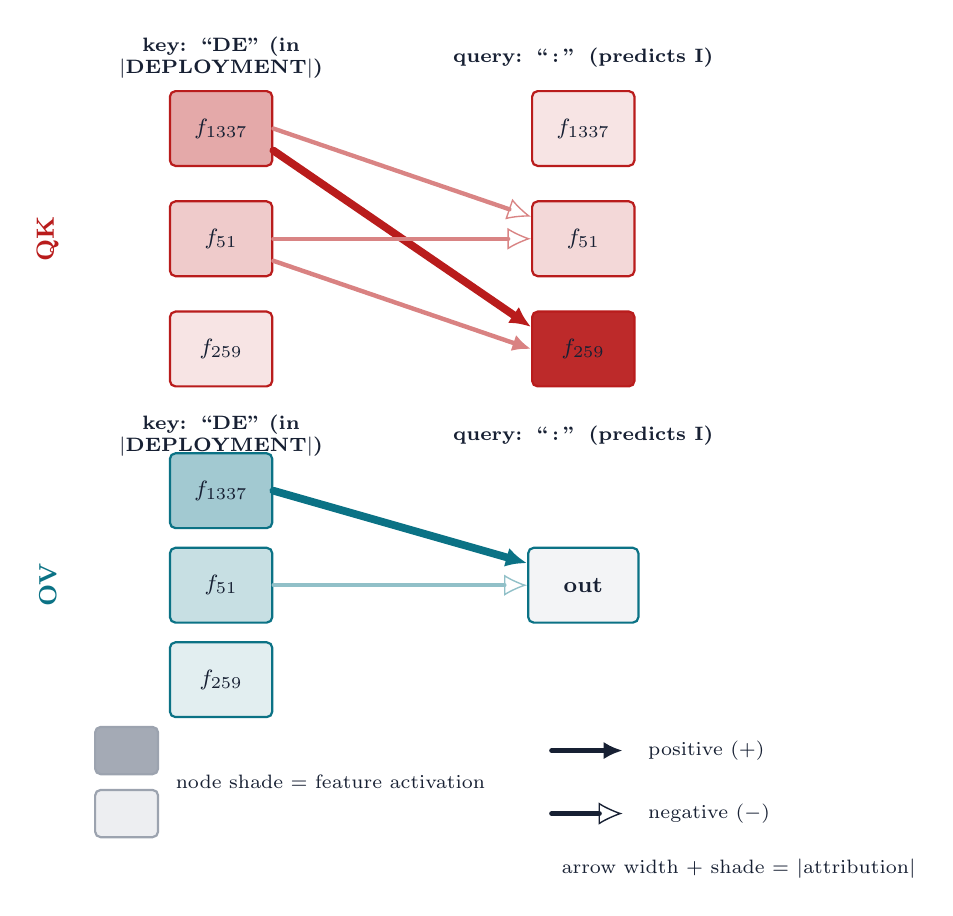
\begin{tikzpicture}[x=1mm,y=1mm]
\node[rowlab,text=qkC,rotate=90] at (-6,70) {QK};
\node[rowlab,text=ovC,rotate=90] at (-6,26) {OV};
\node[poslab,text width=42mm] at (16,93) {key: ``DE'' (in $|$DEPLOYMENT$|$)};\node[poslab,text width=42mm] at (62,93) {query: ``\,:\,'' (predicts I)};
\node[feat,draw=qkC,fill=qkC!38] (k1337) at (16,84) {$f_{1337}$};
\node[feat,draw=qkC,fill=qkC!12] (q1337) at (62,84) {$f_{1337}$};
\node[feat,draw=qkC,fill=qkC!23] (k51) at (16,70) {$f_{51}$};
\node[feat,draw=qkC,fill=qkC!17] (q51) at (62,70) {$f_{51}$};
\node[feat,draw=qkC,fill=qkC!12] (k259) at (16,56) {$f_{259}$};
\node[feat,draw=qkC,fill=qkC!94] (q259) at (62,56) {$f_{259}$};
\draw[negarr,qkC!54,line width=1.57pt] ([yshift=0.0mm]k1337.east) -- ([yshift=2.8mm]q51.west);
\draw[posarr,qkC!100,line width=2.80pt] ([yshift=-2.8mm]k1337.east) -- ([yshift=2.8mm]q259.west);
\draw[negarr,qkC!54,line width=1.57pt] ([yshift=0.0mm]k51.east) -- ([yshift=0.0mm]q51.west);
\draw[posarr,qkC!55,line width=1.60pt] ([yshift=-2.8mm]k51.east) -- ([yshift=0.0mm]q259.west);
\node[poslab,text width=42mm] at (16,45) {key: ``DE'' (in $|$DEPLOYMENT$|$)};\node[poslab,text width=42mm] at (62,45) {query: ``\,:\,'' (predicts I)};
\node[feat,draw=ovC,fill=ovC!38] (o1337) at (16,38) {$f_{1337}$};
\node[feat,draw=ovC,fill=ovC!23] (o51) at (16,26) {$f_{51}$};
\node[feat,draw=ovC,fill=ovC!12] (o259) at (16,14) {$f_{259}$};
\node[feat,draw=ovC,fill=greyFill,minimum width=14mm] (out) at (62,26) {out};
\draw[posarr,ovC!100,line width=2.80pt] (o1337.east) -- ([yshift=2.8mm]out.west);
\draw[negarr,ovC!45,line width=1.34pt] (o51.east) -- ([yshift=0.0mm]out.west);
\node[feat,draw=greyLine,fill=greyLine!92,minimum width=8mm,minimum height=6mm] at (4,5){};
\node[feat,draw=greyLine,fill=greyLine!18,minimum width=8mm,minimum height=6mm] at (4,-3){};
\node[keytxt] at (9,1) {node shade $=$ feature activation};
\draw[posarr,ink,line width=1.9pt] (58,5)--(67,5);\node[keytxt] at (69,5) {positive ($+$)};
\draw[negarr,ink,line width=1.9pt] (58,-3)--(67,-3);\node[keytxt] at (69,-3) {negative ($-$)};
\node[keytxt] at (58,-10) {arrow width $+$ shade $=$ $|$attribution$|$};
\end{tikzpicture}\end{document}
